\chapter{Einleitung}
\label{ch:einleitung}

\section{Motivation/Aufgabe}
Ziel des Versuches ist die Untersuchung des Absorptionsverhaltens einer Kaliumpermanganat-Lösung ({KMnO4}). Dabei wird das Absorptionsspektrum aufgenommen und der molare Extinktionskoeffizient~$\varepsilon$ bestimmt. Zur Bestimmung werden zwei Verfahren angewendet, die auf dem Lambert'schen Absorptionsgesetz und dem Beer'schen Gesetz beruhen. Im ersten Verfahren wird die Abhängigkeit der Lichtabsorption von der Schichtdicke~$l$ untersucht, im zweiten die Abhängigkeit von der Konzentration~$c$. Beide Methoden erlauben die experimentelle Ermittlung von~$\varepsilon$ bei einer Wellenlänge von $\lambda = 525\,\text{nm}$.

\section{Physikalische Grundlagen}
\subsection*{Fotometrie}
Die Fotometrie beschreibt die Bestimmung der Konzentration einer Substanz durch Messung der Lichtabsorption. Trifft Licht mit einer Anfangsintensität~$I_0$ auf ein absorbierendes Medium, so nimmt die Intensität~$I$ beim Durchlaufen einer Strecke~$l$ exponentiell ab. Dies wird durch das Lambert'sche Absorptionsgesetz beschrieben:

\begin{equation}
    I = I_0 e^{-kl}
    \label{eq:lambert}
\end{equation}

wobei $k$ die Extinktionskonstante ist. In logarithmischer Form ergibt sich

\begin{equation}
    \ln \left(\frac{I}{I_0}\right) = -kl
    \label{eq:lambert_log}
\end{equation}

Für praktische Anwendungen wird häufig der dekadische Logarithmus verwendet:

\begin{equation}
    \log I = -k'l + \text{const.}
    \label{eq:bunsen}
\end{equation}

mit dem Zusammenhang $k' = \log(e) \cdot k = 0.434\,k$. Der Koeffizient~$k'$ wird als Bunsenscher oder dekadischer Absorptionskoeffizient bezeichnet. Für verdünnte Lösungen gilt das Beer'sche Gesetz:

\begin{equation}
    k' = \varepsilon c
    \label{eq:beer}
\end{equation}

wobei~$\varepsilon$ der molare Extinktionskoeffizient ist, eine stoffabhängige Konstante. Durch Einsetzen von \hyperref[eq:beer]{Gleichung \ref*{eq:beer}} in das Lambert'sche Gesetz \hyperref[eq:lambert]{Gleichung \ref*{eq:lambert}} ergibt sich:

\begin{equation}
    I = I_0 \cdot 10^{-\varepsilon c l}
    \label{eq:combined}
\end{equation}

Die Größen~$k'$ und~$\varepsilon$ sind wellenlängenabhängig und charakterisieren das Absorptionsspektrum eines Stoffes. In einem Absorptionsspektrum werden die Intensität oder der Fotostrom über der Wellenlänge~$\lambda$ aufgetragen. Die Lage der Absorptionsbanden erlaubt die Identifikation bestimmter Ionen und dient der quantitativen Analyse von Lösungen.

\subsection*{Gitterspektrometer}
Zur Messung der spektralen Intensitätsverteilung wird ein Gitterspektrometer verwendet. Dabei wird das Licht durch ein optisches Gitter gebeugt und auf eine CCD-Zeile abgebildet. Unterschiedliche Wellenlängen~$\lambda$ werden aufgrund unterschiedlicher Beugungswinkel räumlich getrennt. Das Spektrometer arbeitet im Bereich von 180\,nm bis 950\,nm mit einer Auflösung von etwa 1\,nm. Über eine Lichtleitfaser wird das Licht eingekoppelt und auf den Sensor geführt. Zur Datenauswertung wird die Software \textit{OceanView} eingesetzt, welche Dunkelstromkorrekturen und Mittelwertbildungen mehrerer Scans ermöglicht. Dadurch werden statistische Fluktuationen reduziert und eine präzise Aufnahme des Absorptionsspektrums gewährleistet.

\begin{figure}[!ht]
    \centering
    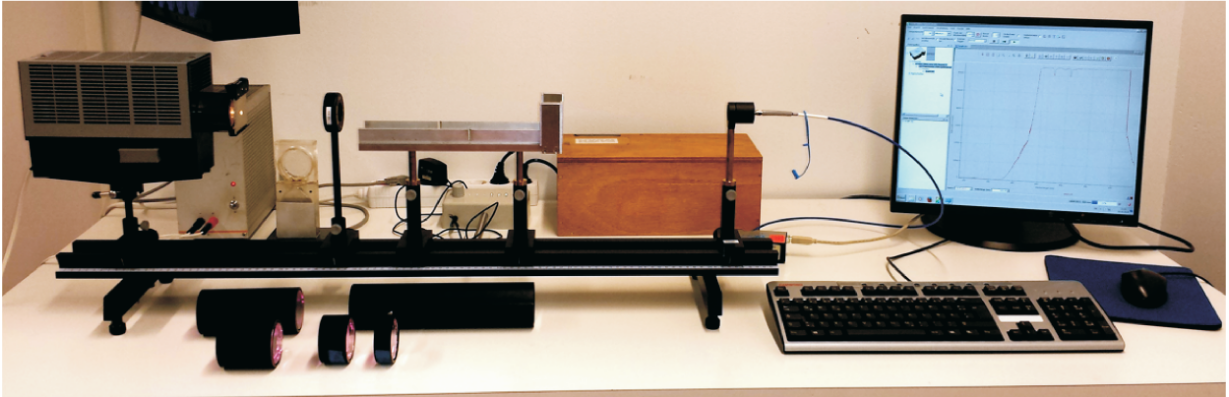
\includegraphics[width=\textwidth]{img/34/Versuchsaufbau.png}
    \caption{Versuchsaufbau \cite{skript25}}
\end{figure}